\section{人口流动网络分析}

\subsection{数据获取}

\begin{frame}[c]{人口流动网络分析(获取)}
    \alert{人口流动}

    \textbf{place/nearby/users}

    \vspace{1em}
    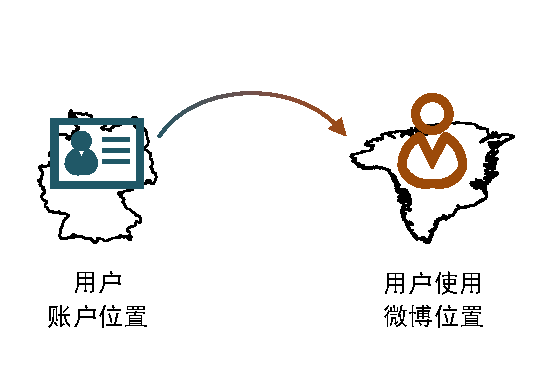
\includegraphics[scale=0.8]{figures/floating.pdf}

\end{frame}

\begin{frame}[t]{人口流动网络分析(获取)}
    \textbf{城市之间GraphX构建}

    \vspace{1em}
    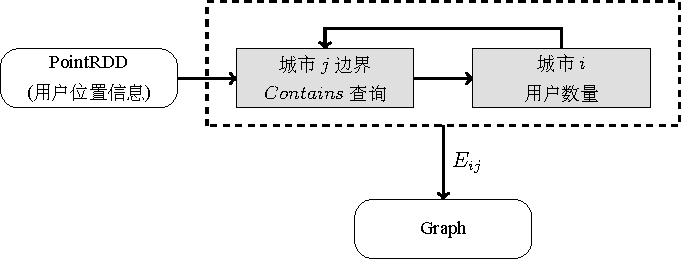
\includegraphics[scale=0.8]{figures/graph.pdf}
\end{frame}

\subsection{统计分析}

\begin{frame}[c]{人口流动网络分析(统计)}
    \begin{columns}
        \begin{column}{0.4 \textwidth}
            人口流动指数

            \begin{itemize}
                \item \textbf{流入量:} $\delta_i$
                \item \textbf{流出量:} $\omega_i$
                \item \textbf{流入流出比:} $\psi_i=\delta_i / \omega_i$
            \end{itemize}
        \end{column}

        % algorithm
        \pause
        \begin{column}{0.6 \textwidth}
            Graph并行化设计, aggreateMessages

            \vspace{0.5em}
            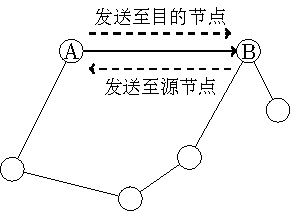
\includegraphics[scale=0.8]{figures/triplet.pdf}
        \end{column}
    \end{columns}
\end{frame}

\begin{frame}[t]{人口流动网络分析(统计)}
    全国城市人口流动情况

    \vspace{0.5em}
    \includegraphics[width=1.0 \linewidth]{figures/flowratio.png}

    \vspace{0.5em}
    \pause
    人口流动量前20\%的城市占全国总流动人口的70.1\%。
\end{frame}
%--- Next Frame ---%

\begin{frame}[t]{人口流动网络分析(统计)}
    人口流入流出比
    
    \begin{itemize}
        \pause
        \item \alert{大于1}

        辽源、鄂州、西双版纳、毕节、永州、七台河、娄 底、姿阳、白色、黄冈、松原、三亚、娄底、大理等

        \pause
        \item \alert{接近1}

        上海、北京、成都、武汉、哈尔滨、嘉兴、杭州、长 沙,广州、西安、太原、郑州、沈阳、乌鲁木齐等

        \pause
        \item \alert{小于1}

        东莞、马鞍山、芜湖、青岛、苏州、深圳、包头、宁 波、无锡、唐山,石家庄、呼和浩特等
    \end{itemize}
\end{frame}
%--- Next Frame ---%

\subsection{流向分析}

\begin{frame}[t]{人口流动网络分析(流向分析)}
    \begin{columns}
        \begin{column}{0.4 \textwidth}
            \alert{流向示意图}

            \begin{figure}
                \includegraphics[scale=0.4]{figures/flow.jpg}
            \end{figure}
        \end{column}

        \pause
        \begin{column}{0.6 \textwidth}
            \textbf{PageRank}计算网络节点的权重

            \begin{enumerate}
                \item 北京 0.058
                \item 成都 0.033
                \item 上海 0.031
                \item 西安 0.028
                \item 广州 0.026
                \item 武汉 0.024
                \item 杭州 0.017
                \item 郑州 0.016
                \item 深圳 0.015
                
                $\ldots$
            \end{enumerate}
        \end{column}
    \end{columns}
\end{frame}


\begin{frame}[t]{人口流动网络分析(流向分析)}
    城市权重与城市GDP相关系数为0.8

    \pause
    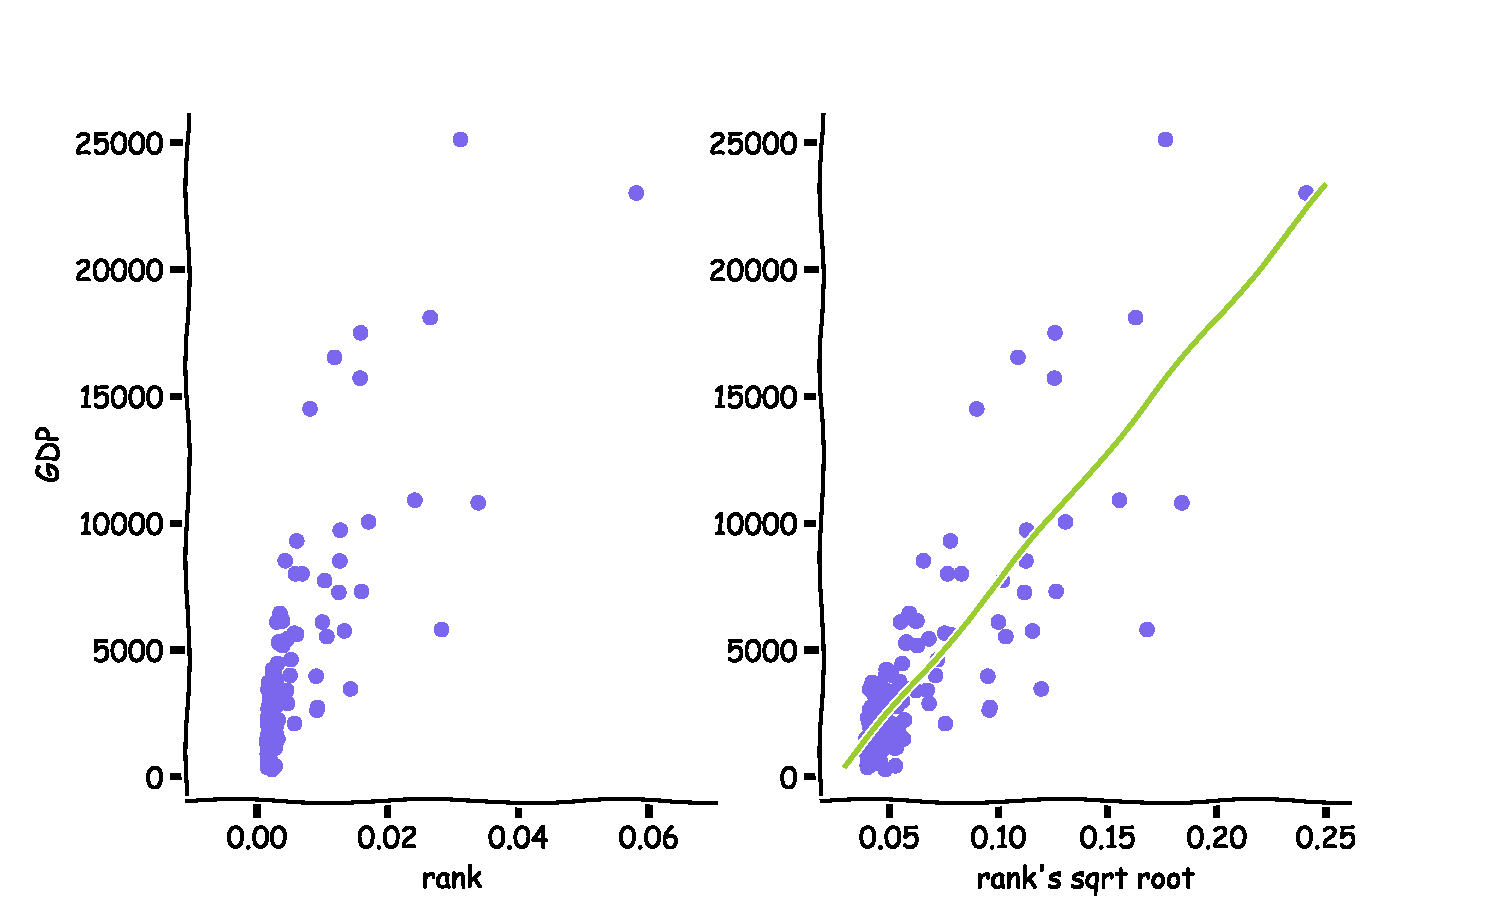
\includegraphics[scale=0.4]{figures/rank_gdp_scatter.pdf}

    $\text{GDP} = 1.037\times 10^5 rank^{0.5}-2669$
\end{frame}

\begin{frame}[t]{人口流动网络分析(流向分析)}
    残差平方与杠杆值散点图

    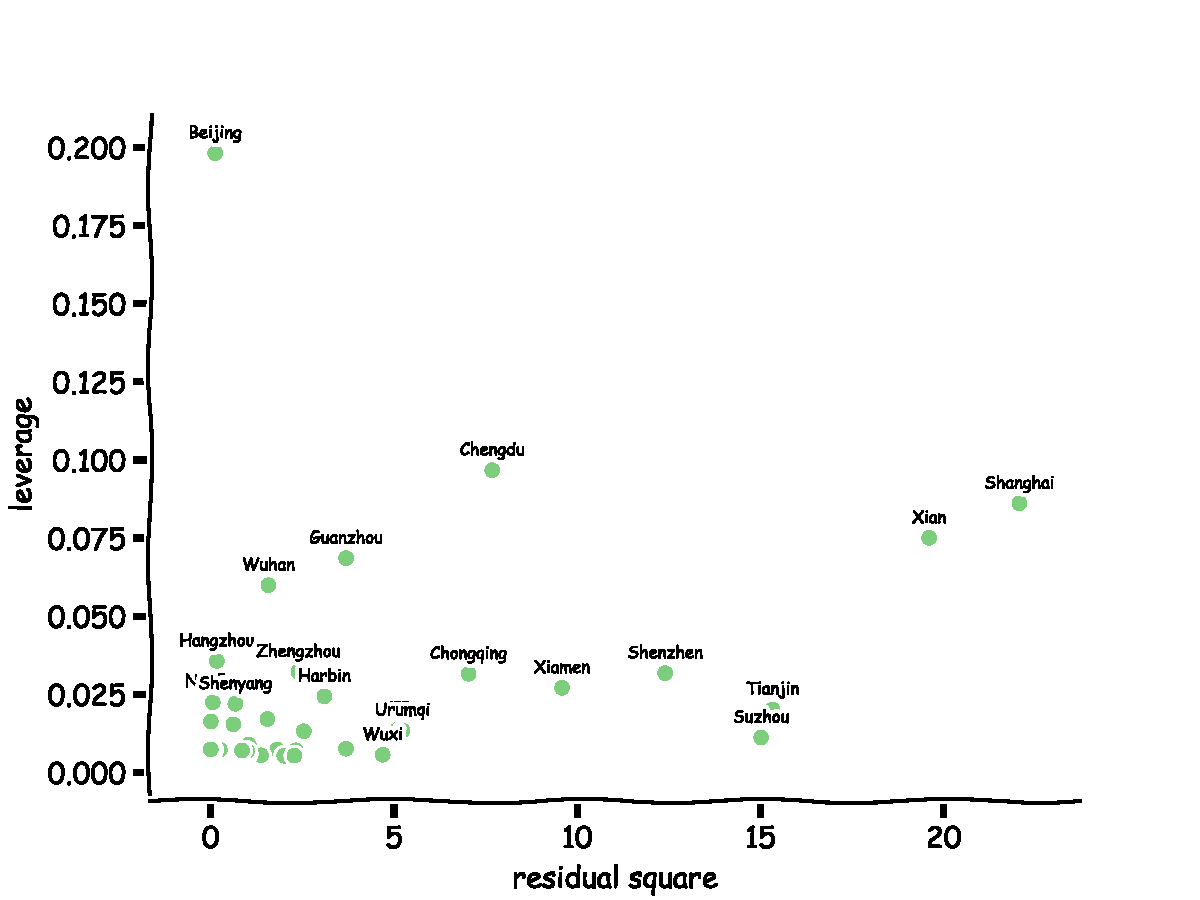
\includegraphics[scale=0.4]{figures/leverage.pdf}
\end{frame}

\begin{frame}[t]{口流动网络分析(流向分析)}
    \alert{结论}

    \begin{enumerate}
        \pause
        \item \textbf{城市权重与城市经济发展相对一致性}

        城市的权重与城市GDP呈现一定的正相关关系,即城市的权重越高,城市的GDP数值会高,但也有异常

        \pause
        \item \textbf{城市权重在流动网络层级分布}

        北京为第一个层级;成都、上海、西安、广州和武汉为第二层级;杭州、郑州、深圳、重庆
        和厦门为第三个层级;哈尔滨、南京、长沙、沈阳和天津为第三层级;

        \pause
        \item \textbf{东部城市与中西部城市权重的差异明显}

        东部城市群在人口流动网络中扮演重要的角色
    \end{enumerate}
\end{frame}
%--- Next Frame ---%



\subsection{社群挖掘}

\begin{frame}[t]{人口流动网络分析(社群挖掘)}
    \small

    \begin{alert}{模块值}
        \begin{equation}
            Q=\frac{1}{2m}\displaystyle{\sum_{vw}\big(W_{vw}-P_{vw}\delta(C_v,C_w)\big)}
        \end{equation}
    \end{alert}
    其中$W_{vw}$为网络中节点$v$和节点$w$之间的权重;$m$为权重之和;$P_{vw}$为零模型中节点之间的期望权重;$C_v$表示节点$v$所属的社群
的类别,如果节点$v$和节点$w$所属同一个社群,则$\delta(C_v,C_w)$为1,否则为0

    \begin{alert}{模块值更新}
        \begin{equation}
        \Delta Q_{AB}=Q_{AB}-Q_{A}-Q_{B}=\frac{1}{2m}\displaystyle{\sum_{a_i \in A, b_j \in B}}\bigg\{ \big( A_{ij} - \frac{k_ik_j}{2m} 
        \big) \times \delta \big[ r(i),r(j) \big] \bigg\}
        \end{equation}
    \end{alert}
%     将复杂网络划分若干个子社群

%     \pause
%     \alert{模块值法}

%     \begin{equation}
%         Q=\frac{1}{2m}\displaystyle{\sum_{vw}\big(W_{vw}-P_{vw}\delta(C_v,C_w)\big)}
%     \end{equation}

%     其中$W_{vw}$为网络中节点$v$和节点$w$之间的权重;$m$为权重之和;$P_{vw}$为零模型中节点之间的期望权重;$C_v$表示节点$v$所属的社群
% 的类别,如果节点$v$和节点$w$所属同一个社群,则$\delta(C_v,C_w)$为1,否则为0。

%     \pause
%     \alert{模块值更新}

%     \begin{equation}
%         \Delta Q_{AB}=Q_{AB}-Q_{A}-Q_{B}=\frac{1}{2m}\displaystyle{\sum_{a_i \in A, b_j \in B}}\bigg\{ \big( A_{ij} - \frac{k_ik_j}{2m} 
%         \big) \times \delta \big[ r(i),r(j) \big] \bigg\}
%     \end{equation}
\end{frame}
%--- Next Frame ---%

\begin{frame}[t]{人口流动网络分析(社群挖掘)}
    \emph{改进}

    \begin{equation}
        Q=\sum_{c}\big\{\frac{\sum_{in}}{2m} - (\frac{\sum_{tot}}{2m})^2\big\}
    \end{equation}

    其中$\sum_{in}$是社群$c$内部相互连接权重和,$\sum_{tot}$该社群$c$外部连接权重和

    \pause

    \begin{equation}
        \Delta Q=\big[ \frac{\sum_{in} + k_{i,in}}{2m} -(\frac{\sum_{tot}+k_i}{2m})^2 \big] 
            - \big[ \frac{\sum_{in}}{2m} - (\frac{\sum_{tot}}{2m})^2 - (\frac{k_i}{2m})^2 \big]
    \end{equation}

\end{frame}
%--- Next Frame ---%

\begin{frame}[t]{人口流动网络分析(社群挖掘)}

    \begin{algorithm}[H]
    \tiny
\caption{社群挖掘算法}
\begin{algorithmic}[1]
\REQUIRE ~~\\
网络图:graph; \\
最多迭代次数: maxIterations;\\
模块值变化阈值: modularityThreshold;\\
\ENSURE ~~\\
模块值最大社群图: graph; \\
\STATE 初始化$C_i,\{i=1, 2,\ldots , N\}$
\STATE iterate=0
\WHILE{changeRate<modularityThreshold || iteration < maxIterations}
    \STATE changeRate=0
    \FORALL{$i$ in graph.vertexs} 
    \STATE $Q_i=[\quad ]$
    \FORALL{$j$ in $i$ neighbors}
    	\STATE $Q_i$ += $\Delta Q(i,j)$ $//$计算模块值增益
    \ENDFOR
    \STATE $Q_{max}$=max($Q_i$)
    \IF {$Q_{max} > 0$}
    	\STATE graph=updategraph() $//$如果最大模块值增益大于零,合并顶点
	\STATE changeRate= $Q_{max}$
    \ENDIF
    \ENDFOR
 \STATE iterate += 1 \\
\ENDWHILE
\RETURN graph
\end{algorithmic}
\end{algorithm}
\end{frame}
%--- Next Frame ---%

\begin{frame}[t]{人口流动网络分析(社群挖掘)}
    并行化设计,aggregateMessages接口
    \begin{enumerate}

    \pause 
    \item \textbf{map阶段}

    消息类,包含了顶点、所属社群和目标社群的权重

    \pause
    \item \textbf{Reduce阶段}

    将发送到同一个顶点的消息按照模块增益值最大进行合并

    \pause
    \item \textbf{连通量合并}

    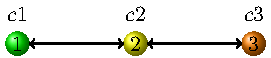
\includegraphics[scale=0.8]{figures/communitycombine.pdf}

    \pause
    \item \textbf{图更新}
    
    与上一轮的Graph对象的顶点进行joinVertice操作

    \end{enumerate}

\end{frame}
%--- Next Frame ---%

\begin{frame}[t]{人口流动网络分析(社群挖掘)}
    全国城市社群划分

    \includegraphics[scale=0.7]{figures/commumity.jpg}
\end{frame}
%--- Next Frame ---%

\begin{frame}[t]{人口流动网络分析(社群挖掘)}
    \alert{社群划分结果}

    \begin{enumerate}
        \item 北京、天津、河北城市、东三省城市、福建城市、三亚等
        \item 山东城市
        \item 河南城市
        \item 山西城市
        \item 湖北城市、江西城市
        \item 上海、江苏城市、安徽城市、浙江城市、丽江
        \item 广东城市、广西城市、湖南城市等
        \item 重庆、四川城市、贵州城市等西南城市
        \item 新疆城市、甘肃城市等西北城市
    \end{enumerate}
\end{frame}
%--- Next Frame ---%

\begin{frame}[t]{人口流动网络分析(社群挖掘)}
    \textbf{结论}

    \begin{enumerate}
        \item 城市之间人口流动以省份为划分的特征较为明显
        \item 城市社群组成受地理空间位置影响较大,有明显的区域特征
        \item 城市社群组成也存在不受地理位置影响的特殊情况,如福建省,三亚市与北方城市组成同一社群,
              丽江与东部省份城市为一个社群。从侧面表明其人口流动突破了地理空间的限制
        \item 当对全国社群进行子社群进行社群挖掘,可以发现以省份为集聚现象越发明显
    \end{enumerate}
\end{frame}
%--- Next Frame ---%